%% This is an example first chapter.  You should put chapter/appendix that you
%% write into a separate file, and add a line \include{yourfilename} to
%% main.tex, where `yourfilename.tex' is the name of the chapter/appendix file.
%% You can process specific files by typing their names in at the 
%% \files=
%% prompt when you run the file main.tex through LaTeX.

\chapter{An improved hidden Markov method for geolocating archival-tagged fishes}
\label{chap:2}
\raggedbottom
%\begin{singlespace}
%Harriet Alexander$^{1,2}$, Bethany D. Jenkins$^{3,4}$, Tatiana A. Rynearon$^{3}$, Mak A. Saito$^{5}$, Melissa L. Mercier$^{3}$, Sonya T. Dyhrman$^{2}$\\
%\\
%$^{1}$ MIT-WHOI Joint Program in Oceanography/Applied Ocean Science and Engineering, Cambridge, MA 02139, USA\\
%$^2$ Biology Department, Woods Hole Oceanographic Institution, Woods Hole, MA 02543, USA\\
%$^3$ Graduate School of Oceanography, University of Rhode Island, Narragansett, RI 02882, USA\\
%$^4$ Department of Cell and Molecular Biology, University of Rhode Island, Kingston, RI 02881, USA\\
%$^5$ Department of Marine Chemistry and Geochemistry, Woods Hole Oceanographic Institution, Woods Hole, MA 02543, USA\\
%\\
{\let\thefootnote\relax\footnotetext{This chapter was originally published as Braun, C.D., Galuardi, B., and Thorrold S.R. (2018). \href{http://onlinelibrary.wiley.com/doi/10.1111/2041-210X.12959/full}{HMMoce: An R package for improved geolocation of archival-tagged fishes using a hidden Markov method.} \emph{Methods in Ecology and Evolution} 9, 1212-1220. }}
%\end{singlespace}
{\let\thefootnote\relax\footnotetext{C.D.B and B.G. conceived the project and developed the package; C.D.B and S.R.T. collected the data; C.D.B. wrote the paper; B.G. and S.R.T. contributed to the writing of the paper.}}
{\let\thefootnote\relax\footnotetext{The supplemental methods, figures, and tables for this chapter can be found in \cref{sec:app2}.}}

\clearpage

\section{Summary}\label{summary}

\begin{enumerate}[itemsep=0.1mm]
\def\labelenumi{\arabic{enumi}.}
\item Electronic tagging of marine fishes is commonly achieved with archival tags that rely on light levels and sea surface temperatures to retrospectively estimate movements. However, methodological issues associated with light-level geolocation have constrained meaningful inference to species where it is possible to accurately estimate time of sunrise and sunset. Most studies have largely ignored the oceanographic profiles collected by the tag as a potential way to refine light-level geolocation estimates.

\item Open-source oceanographic measurements and outputs from high-resolution models are increasingly available and accessible. Temperature and depth profiles recorded by electronic tags can be integrated with these empirical data and model outputs to construct likelihoods and improve geolocation estimates.

\item The \texttt{R} package \texttt{HMMoce} leverages available tag and oceanographic data to improve position estimates derived from electronic tags using a hidden Markov approach. We illustrate the use of the model and test its performance using example blue and mako shark archival tag data. Model results were validated using independent, known tracks and compared to results from other geolocation approaches.

\item \texttt{HMMoce} exhibited as much as 6-fold improvement in pointwise error as compared to traditional light-level geolocation approaches. The results demonstrated the general applicability of \texttt{HMMoce} to marine animals, particularly those that do not frequent surface waters during crepuscular periods.
\end{enumerate}
 
\section{Introduction}
Electronic archival tags have been widely adopted by ecologists to track
movements of wide-ranging species that are difficult to monitor using
other techniques. In ocean environments, implanted archival and pop-up
satellite archival transmitting (PSAT) tags have proved particularly
valuable in the study of life history patterns
\citep[\emph{e.g.}][]{Thorrold2014}, biophysical interactions and habitat use
\citep[\emph{e.g.}][]{Braun2015a, Lam2014}, horizontal and vertical movements
\citep[\emph{e.g.}][]{Braun2014, Lam2016, Werry2014}, and the spatial structure
of populations \citep{Skomal2009, Galuardi2010, Galuardi2014} in a
number of commercially important fishes \citep{Block2011} and species of
conservation concern \citep{Braun2015}. Yet, tracks provided by
electronic tags that rely on light-level geolocation often exhibit large
error in daily position estimates \citep{Musyl2011a, Braun2015a} that
may hinder inferences drawn from the tag data. Approaches that provide
more certainty in movement estimates derived from light level data
\citep{Galuardi2014, Luo2015} would increase the power of ecological
hypotheses tested using tag data.

Electronic archival tags typically use light levels to estimate position
when it is not possible for the tag to interrogate geo-location
satellites \citep{Sibert2003, Nielsen2007}. Accuracy of geolocation
using light levels, however, is limited ($\pm$ 100-200 km;
$\sim$10,000 km$^2$) even for surface-oriented
species where good light data is available
\citep{Wilson2007, Braun2015a}. While several studies have incorporated
ancillary data, including sea surface temperature
\citep{Smith1986, Lam2010}, tidal fluctuation \citep{Pedersen2008} or
ocean heat content \citep{Luo2015} to help improve geolocation
estimates, only one used all data collected from archival tags within a
rigorous statistical framework to improve geolocation estimates
\citep{Sumner2009}. Although excursions from the photic zone, including
diel vertical migration \citep{Neilson2009} and extended mesopelagic
occupation \citep{Skomal2009} may render light geolocation impossible,
the depth-temperature profiles recorded by the tags provide diagnostic
oceanographic signatures that can be leveraged to help constrain
position \citep{Skomal2009, Aarestrup2009}.

Hidden Markov Models (HMMs) have gained popularity in recent years as a
tool for analyzing animal movement data and have been applied to
understand movements of a number of organisms
\citep{Holzmann2006, Thygesen2009a, Pedersen2011}. Much of the progress
in ocean environments stems from a HMM used to track cod in the North
Sea using tidal information \citep{Pedersen2008}. The approach combined
a number of desirable features, including inference about the underlying
behavioral state of the animal, mobilization of oceanographic data in a
spatial likelihood framework \citep{Nielsen2006}, and later incorporated
formal treatment of barriers to movement \citep{Pedersen2011}.
Generally, the Bayesian HMM approach uses a model of animal movements
(\emph{e.g.}~Brownian motion) and a model or observations of the environment
(\emph{e.g.}~in situ oceanography) to estimate the posterior distribution of
the state (\emph{e.g.}~animal position and behavior). Several \texttt{R}
packages exist for analyzing movement data with HMMs, including
\texttt{ctmm} \citep{Calabrese2016} and \texttt{moveHMM}
\citep{Michelot2016}, but none are designed for geolocating marine
fishes with archival tag data. An electronic tag manufacturer (Wildlife
Computers, Inc.) recently updated their proprietary software (GPE3) to
geolocate archival tag data based on light levels and sea surface
temperature (SST) in a HMM framework following \citet{Pedersen2008}.
However, GPE3 is limited by a lack of behavior state-switching dynamics
and does not include functionality for non-surface oriented species.
GPE3 is also proprietary software that cannot be modified by the user
and is limited to tags built by Wildlife Computers.

Our primary objective was to build an analysis toolkit to improve
geolocation estimates from electronic archival tags deployed on marine
animals that alleviates many of the limitations imposed by previous
approaches. The new \texttt{R} package \texttt{HMMoce} uses available
electronic tag data and oceanographic data mined from ocean observing
system portals to estimate animal movements, behavior, and residency
from uncertain and temporally correlated movement data. We modify and
expand a hidden Markov approach
\citep{Thygesen2009a, Pedersen2008, Pedersen2011} that, in addition to
estimating animal movements, allows behavior state estimation and
provides information about the posterior distribution of the modeled
states that can be used as a residency metric \citep{Pedersen2011}. The
modeling framework we developed is sufficiently flexible to accommodate
other tag types and animal movement questions, can be applied in any
geographic location, and benefits from the transparency of a widely-used
open source platform. Here we describe the model framework and
demonstrate its applicability using example data. For specific details
on package use and functions and a full tutorial with an example
dataset, please refer to the package and its accompanying vignette,
available on CRAN.

\section{Overview of HMMoce}

\subsection{Model formulation}

We present a process-based approach to estimate residency and behavior
from movement data collected with electronic archival tags. The logic of
this approach involves calculating gridded observation likelihoods at
each time point based on tag and environmental data, forming the
state-space model, estimating model parameters and model selection and
interpretation. The application of grids to explicitly resolve space is
a key component that allows state estimation (location and behavior, in
this case) to be supplemented by or based entirely on environmental data
(\emph{e.g.}~temperature at depth). The details of the discretized grid HMM
approach are thoroughly explained elsewhere
\citep[\emph{e.g.}][]{Thygesen2009a, Pedersen2011}. A detailed methodology for
our approach can be found in the Appendix \ref{sec:app2}.

\begin{table}[b] % tag summary
\centering
\caption[Satellite tagging summary for \texttt{HMMoce} model data]{Tagging summary for double-tagged blue (BSH) and shortfin mako (MKO) sharks used in this study.}
\label{tab:c2t1}
\small
%\begin{tabular}[t]{lrllrrrrr}
\begin{tabular}{p{1.25cm} p{1.25cm} p{2cm} p{2cm} p{1.5cm} p{1.25cm} p{1cm} p{1cm} p{1cm}}
\toprule
\textbf{Species} & \textbf{Tag ID} & \textbf{Start Date} & \textbf{End Date} & \textbf{Duration (d)} & \textbf{PDT (\%)} & \textbf{Light (\%)} & \textbf{SST (\%)} & \textbf{SPOT (\%)}\\
\midrule
BSH & 141254 & 2015-10-21 & 2016-02-05 & 107 & 72 & 100 & 92 & 96\\
BSH & 141256 & 2015-10-13 & 2016-02-24 & 134 & 66 & 94 & 88 & 87\\
BSH & 141259 & 2015-10-13 & 2016-04-10 & 180 & 53 & 94 & 82 & 85\\
MKO & 141257 & 2015-10-15 & 2016-04-12 & 180 & 58 & 96 & 69 & 72\\
\bottomrule
\end{tabular}
\caption*{PDT, Light, SST and SPOT = percent of deployment period with depth-temperature profile (PDT), light and sea surface temperature (SST) data from the PSAT tag and percent of deployment period with Argos-based positions (SPOT), respectively.}
\end{table}

%Figure 1: example PDT data
\begin{figure}[p]
\centering
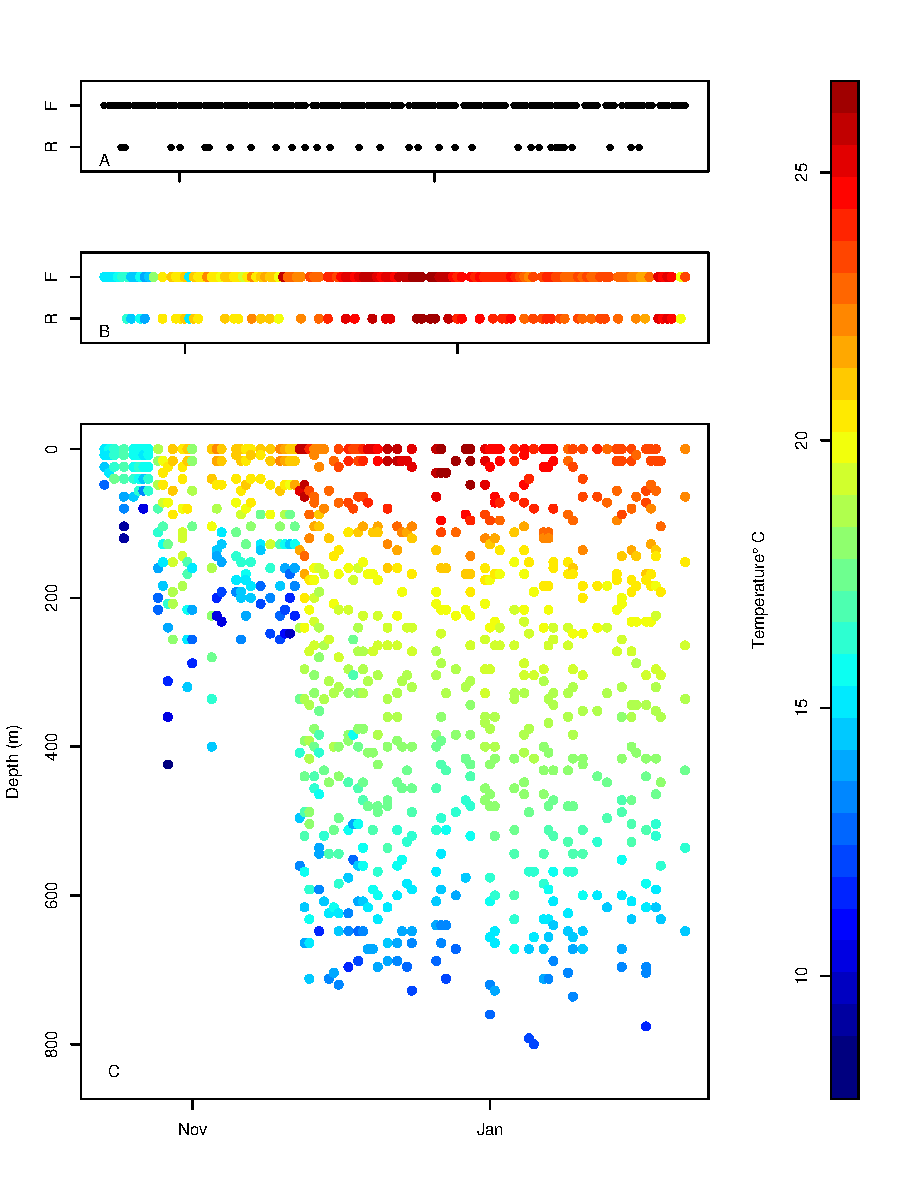
\includegraphics[width=1\textwidth]{images/C2_Fig1.pdf}
\caption[Example pop-up satellite archival tag data]{Example blue shark data demonstrating the deployment days with
(A) light, (B) sea surface temperature and (C)
depth-temperature profile data used as the observation portion of the
HMM. Full [F] and removal [R] datasets for light and SST are shown
(A,B).}
\label{fig:c2f1}
\end{figure}

Briefly, observation-based likelihoods (Eq. \ref{eq:a1e1}) were derived from \is SST (Eq. \ref{eq:a1e2}), light-based longitude and depth-temperature profile
data (Eq. \ref{eq:a1e3}, \ref{eq:a1e4}, \ref{eq:a1e5}) collected by the tags using five separate
likelihood calculations: \emph{1)} An SST likelihood (Eq. \ref{eq:a1e2}) was
generated for tag-based SST values integrated according to an error term
($\pm$ 1\%, based on tag sensor accuracy) and compared to
remotely-sensed SST from daily, optimally-interpolated SST fields
\citep[OI-SST, 0.25$^{\circ}$ resolution;][]{Banzon2016}. \emph{2)} Light-based
longitude likelihood was derived using estimates of longitude from GPE2
software (Wildlife Computers, Inc.), which facilitated visual checking
of light curves. Depth-temperature profiles recorded by the tag were
compared to \emph{3)} monthly climatological mean depth-temperature data
from the World Ocean Atlas 2013 \citep[WOA, 0.25$^{\circ}$
resolution;][]{Locarnini2013} and \emph{4)} daily reanalysis model
depth-temperature products from the HYbrid Coordinate Ocean Model
\citep[HYCOM, 0.08$^{\circ}$ resolution;][]{Chassignet2007} at standard depth
levels available in these products (Eq. \ref{eq:a1e5}). Individual likelihood
surfaces for each depth level were then combined for an overall profile
likelihood at that time point (Eq. \ref{eq:a1e6}). \emph{5)} Ocean Heat Content
(OHC)(Eq. \ref{eq:a1e5}) was obtained by integrating the heat content of the water
column above the minimum daily temperature recorded by the tag for both
the tag profiles and HYCOM fields \citep[Eq. \ref{eq:a1e4};][]{Luo2015}. Start and
end locations were considered known in all cases and model runs.

The resulting observation likelihoods (in various combinations; Eq. \ref{eq:a1e1})
were used in a two-step Bayesian state-space approach to estimate the
posterior distribution of the state (in this case, a joint probability
distribution of location and behavior at each time point). Probability
distributions were first calculated forward in time using alternating
time and data updates of the current state estimate using a HMM filter
\citep[for a detailed methodology of the HMM filter see Appendix 2
in][]{Pedersen2011}. The filter recursions also returned a likelihood
measure indicating how well the model fit the data, which facilitated
calculating model parameters (\emph{e.g.}~behavior state-switching
probabilities). In Bayesian statistics, the maximum a priori (MAP)
estimate of the model parameters is typically used to calculate the
posteriors; however, in practice, ample a priori information is rarely
available and maximum likelihood (ML) estimates are often very similar
to MAP estimates \citep{Jonsen2005}. Thus, we implemented recent
advances by \citet{Woillez2016} that further exploited the
discretization of space in this model by employing a joint ML estimation
of all model parameters using an iterative Expectation-Maximization
framework.

Model selection in this context would typically use Bayesian Information
criterion (BIC), but this approach requires approximation that imposes
restrictions on the priors. Instead, we used Akaike's Information
criterion (AIC) for model selection following \citet{Pedersen2011}. The
HMM smoother recursion was the final step that worked backwards in time
using filtered state estimates and all available observation data to
determine smoothed state estimates. This step provided the time marginal
of the probability distributions based on observations (posterior
distributions).

Results from the final smoothing step represent the posterior
distribution of each state over time. Distributions are summed for each
behavior state and time step to determine the most likely behavior state
through time. \texttt{HMMoce} can calculate the mean or mode of the
posterior distribution grid, at each time step, to estimate the animal's
position. The posteriors can be further analyzed for additional
inference including uncertainty and residency. A residency distribution
(RD) is conceptually similar to the utilization distribution (UD), but
the concept of UD (and other space-use metrics) is often vaguely defined
\citep{Royle2008}. In this case, RD is interpreted as the estimate of
the time spent in a given space within a time interval \citep[see Eq. 5
in][]{Pedersen2011}.

%Figure 2: All track comparison
\begin{figure}[p!]
\centering
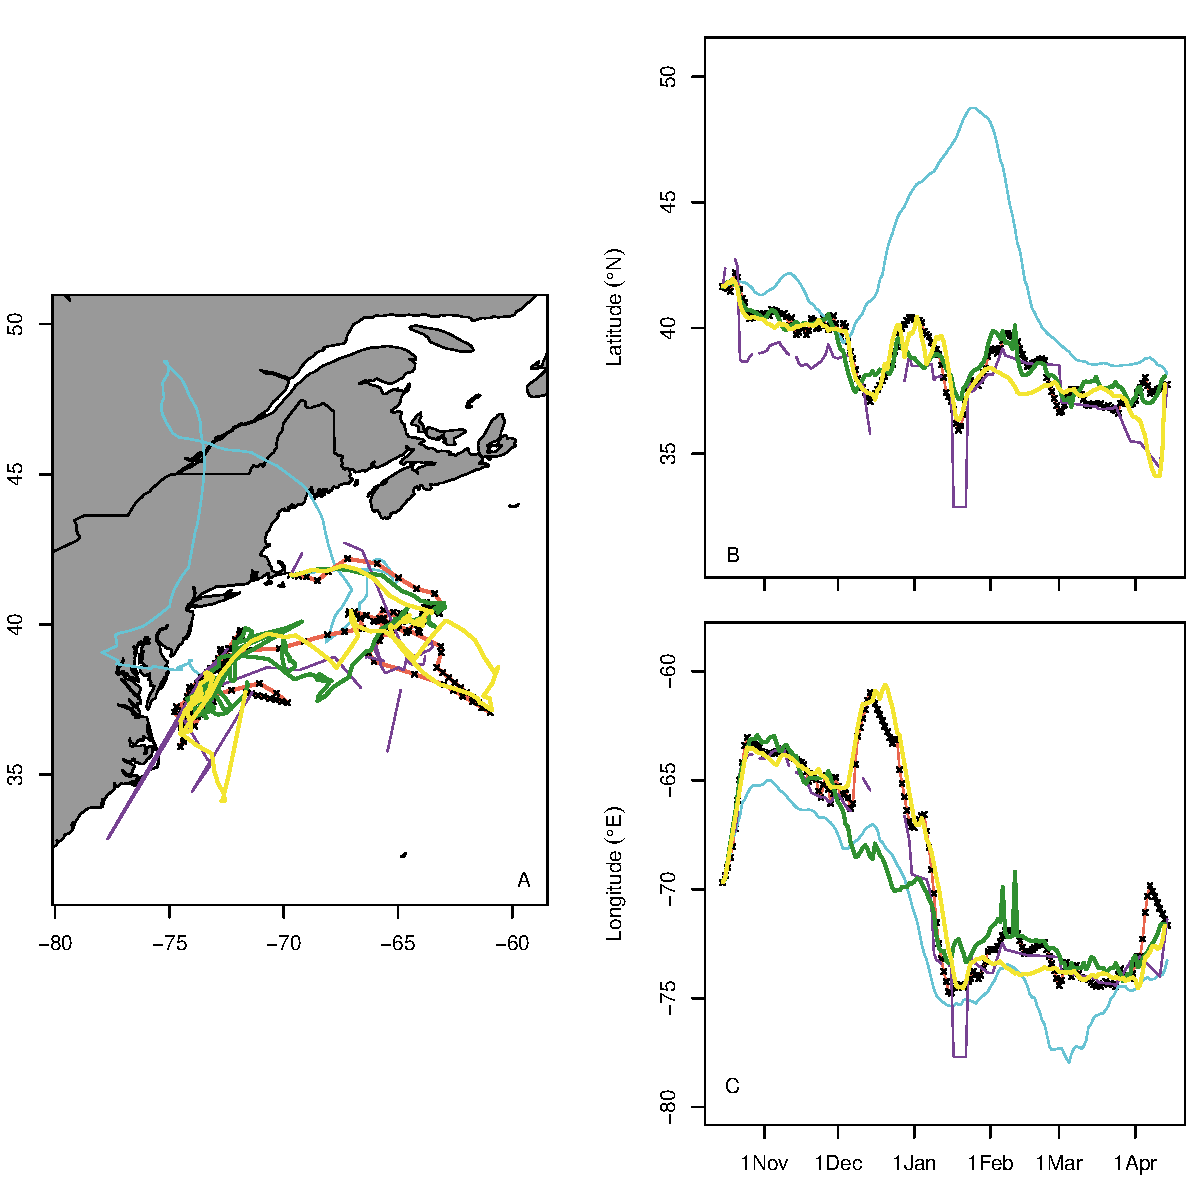
\includegraphics[width=1\textwidth]{images/C2_Fig2.pdf}
\caption[Comparison of results from various geolocation approaches]{Calculated tracks for mako shark 141257 using the 4 different
geolocation approaches (Ukfsst, purple; Trackit, blue; GPE3, green;
\texttt{HMMoce}, yellow) compared to the "known" Argos-based track
(red, black crosses). Latitudinal and longitudinal estimates through
time are shown in panels B and C, respectively. Lines appear broken when
a resulting track is missing daily data.}
\label{fig:c2f2}
\end{figure}

\subsection{Computational improvements and
requirements}

While the basic framework of \texttt{HMMoce} was based on previous work
\citep{Pedersen2008, Thygesen2009a, Pedersen2011}, several improvements
were made to accommodate user needs. We focused several enhancements on
improving computation efficiency, which was a limitation of previous
techniques \citep[\texttt{SPHMM} code for \texttt{R};][]{Pedersen2011}.
Image processing routines replaced sparse matrix convolution yielding
orders of magnitude improvements in computation time, particularly for
large, high-resolution grids that characterize geolocation approaches
for highly migratory species. In addition, all likelihood routines
(except simple light-based likelihood calculations) were parallelized,
yielding marked performance improvements, particularly for likelihoods
comparing 3D depth-temperature profiles to high-resolution 3D HYCOM
grids.

Despite these improvements, \texttt{HMMoce} remains relatively
computationally intensive; however, cloud computing is becoming more
inexpensive and accessible to a broad user group. The \texttt{HMMoce}
package includes a vignette demonstrating simple plug and play
functionality for the model using Amazon Web Services's computational
resources and an associated machine image containing RStudio Server and
all the required dependencies for running \texttt{HMMoce} with
user-provided tag data.

\begin{table}[h!] % error metrics
\caption[Validation metrics for geolocation methods]{Validation metrics for double-tagged
blue (BSH) and shortfin mako (MKO) shark tracks estimated using HMMoce,
GPE3, Trackit (TI) and Ukfsst.}
\label{tab:c2t2}
\centering
\begin{tabular}[t]{lrllrlll}
\toprule
\textbf{Species} & \textbf{Tag ID} & \textbf{Type} & \textbf{Mean (SD)} & \textbf{Median} & \textbf{Range} & \textbf{RMSE} & \textbf{Input}\\
\midrule
BSH & 141254 & HMMoce & 117.4(96.7) & 92.4 & 0.5-443.6 & 1.21, 0.81 & LSO\\
 &  & GPE3 & 175.8(117.1) & 164.3 & 3.2-424.7 & 1.4, 1.64 & LS\\
 &  & TI & 162.3(71.6) & 158.2 & 1-328.2 & 0.97, 1.65 & L\\
 &  & KF & 179.5(99.5) & 178.5 & 1-435.2 & 1.29, 1.24 & L\\
 &  & HMMoce.r & 131.2(96.2) & 101.9 & 0.5-440.5 & 1.23, 1.01 & LS\\
 &  & GPE3.r & 157.6(100.6) & 143.5 & 1.4-408.9 & 1.25, 1.44 & LS\\
\addlinespace
BSH & 141256 & HMMoce & 83.8(63) & 63.7 & 4.9-297.4 & 0.52, 0.93 & LSH\\
 &  & GPE3 & 84.9(68.8) & 66.9 & 5.9-345 & 0.66, 0.89 & LS\\
 &  & TI & 474.2(244.1) & 459.9 & 0-854.3 & 1.98, 4.84 & L\\
 &  & KF & 192.7(152.4) & 172.6 & 0-699.8 & 1.35, 0.65 & L\\
 &  & HMMoce.r & 93.4(57.8) & 79.1 & 4.2-286 & 0.59, 0.92 & LSH\\
 &  & GPE3.r & 423.5(432) & 197.8 & 2.1-1394 & 4.25, 3.96 & LS\\
\addlinespace
BSH & 141259 & HMMoce & 179.4(126) & 150.3 & 4.4-575.2 & 1.79, 1 & LS\\
 &  & GPE3 & 158.1(109.6) & 139.5 & 4.9-434.5 & 1.44, 1.17 & LS\\
 &  & TI & 367.5(239.1) & 291.4 & 2.4-861.5 & 3.3, 2.36 & L\\
 &  & KF & 245.8(225.5) & 194.5 & 1.7-1078.7 & 2.31, 0.88 & L\\
 &  & HMMoce.r & 183.3(132.2) & 140.5 & 4.4-560.5 & 1.9, 0.88 & LS\\
 &  & GPE3.r & 198(129.5) & 162.0 & 6.1-625.8 & 1.61, 1.77 & LS\\
\addlinespace
MKO & 141257 & HMMoce & 99.8(90.7) & 66.8 & 3.8-426.9 & 0.92, 0.99 & LSH\\
 &  & GPE3 & 151.1(161.1) & 93.0 & 6.8-675.2 & 0.65, 2.38 & LS\\
 &  & TI & 462.6(347.7) & 320.5 & 0-1332.7 & 4.6, 2.79 & L\\
 &  & KF & 220.4(151.2) & 173.7 & 0-614.6 & 1.3, 1.32 & L\\
 &  & HMMoce.r & 157.9(128.2) & 119.1 & 3.8-494.4 & 1.05, 1.92 & LSH\\
 &  & GPE3.r & 182.3(171.8) & 136.4 & 0.3-711.2 & 0.88, 2.62 & LS\\
\bottomrule
\end{tabular}
\caption*{Reported error values (mean, sd, median, range) are pointwise distance calculations (mean great circle distance) from known positions (km). Root-mean-square errors (RMSE) are Lat, Lon (degrees). HMMoce.r and GPE3.r indicate fit metrics for data removal experiments in which 75\% of daily light and 50\% of daily SST data was randomly removed. Input indicates input data type: light (L), SST (S), ocean heat content (O), World Ocean Atlas profiles (W) and HYCOM profiles (H). All runs were performed on a 0.08$^{\circ}$ grid with fixed
migratory speed of 2 $m \cdot s^{-1}$ (except 141259 used 4 $m \cdot s^{-1}$).}
\end{table}

\section{Case study: pelagic shark
movements}

To illustrate the application of \texttt{HMMoce}, we analyzed tag data
from three blue sharks (\emph{Prionace glauca}) and one shortfin mako
(\emph{Isurus oxyrinchus}) that were double-tagged with satellite-linked
radio telemetry tags (Wildlife Computers finmount SPOT5 tags) and PSAT
tags (\cref{tab:c2t1}). Full tagging methods are provided in Appendix \ref{sec:app2}. We considered the resulting Argos-based tracks as "known"
because errors on geolocation estimates from the SPOT tags are much
lower \citep[typically \textless{} 10 km;][]{Witt2010, Patterson2010}
than PSAT-based outputs \citep[\textgreater{} 50 km;][]{Winship2012}.
The PSAT tags were deployed for an average of 150 days (range 107-180)
in the northwest Atlantic with overall movements of 5,403-12,122 km. The
PSAT data contained depth-temperature profiles for 53-72\% of days at
liberty and SPOT locations were recorded for 72-96\% of deployment days
(\cref{tab:c2t1})

Blue sharks made frequent dives to the mesopelagic zone
($\sim$600-800 m, max 680-1,688 m) but also frequented the
surface-air interface where the PSAT tags collected good quality light
and SST data (94-100\% deployment days with light, 82-92\% SST)(\cref{fig:c2f1}). The mako occupied a restricted area
($\sim$200 km latitudinal distance) near Cape Hatteras during
the winter months and spent relatively little time far from the edge of the continental shelf compared to the more nomadic blue sharks. The mako
also had high quality light and SST data (96\% and 69\%, respectively)
while regularly diving shallower than the blue sharks
($\sim$400 m). Consistent exposure of the dorsal fin allowed
the SPOT tag to acquire Argos positions throughout the duration of each
deployment (\cref{tab:c2t1}).

We calculated movements of the sharks from PSAT tag data using three
modeling approaches that are currently available (Ukfsst, Trackit, GPE3)
and \texttt{HMMoce} (\cref{sec:app2}). Results for the mako are shown in the
main text (\cref{fig:c2f2}), and blue shark figures are
provided in the supplement (\cref{fig:a1f2}, \cref{fig:a1f3}, \cref{fig:a1f4}). In general,
\texttt{HMMoce} and GPE3 produced the most accurate tracks while those
from Ukfsst and Trackit were often unrealistic with errors as high as
> 1,300 km (\cref{tab:c2t2}). For 3 of 4 individuals, \texttt{HMMoce}
tracks had the lowest pointwise error and correspondingly lowest
root-mean-square error (RMSE) values. For the fourth individual (blue
shark 141259), the mean error and RMSE in latitude for GPE3 ouput was
lower than \texttt{HMMoce}, which had a lower RMSE in longitude. The
traditional approaches (light only, Trackit; light and SST, Ukfsst)
yielded much larger error than \texttt{HMMoce} in all cases and only one
Trackit output (blue shark 141254 without SST) exhibited marginally
smaller error than GPE3 (with SST). In 3 of 4 cases, \texttt{HMMoce}
demonstrated the best fitting model by leveraging either OHC (n=1) or
HYCOM profiles (n=2) (\cref{tab:c2t2}) in addition to light-based longitude and
SST data used in the other geolocation approaches. The movements of blue
shark 141259, in which the \texttt{HMMoce} model did not use
profile-based observations to build the final estimated track, included
time in both dynamic Gulf Stream water and the more homogenous Sargasso
Sea. It proved difficult in both areas to match water column profiles
recorded by the tag (or integrated OHC) with an accurate and constrained
position in the climatological (WOA) or model-based (HYCOM)
oceanographic data (\cref{fig:a1f5}).

While \texttt{HMMoce} was designed to improve geolocation estimates for
all tagged marine organisms, the main impetus for the work was to
fulfill a need for improving track estimates in cases where light and
SST data were lacking due to minimal surface occupation. We tested the
ability of \texttt{HMMoce} to recover accurate tracks with only limited
light-level data by randomly removing (using \texttt{sample} in base
\texttt{R}, without replacement) 75\% and 50\% of deployment days with
adequate light and SST data, respectively, from the shark PSAT data
while keeping the depth-temperature profile data for these days. The
removals approximated PSAT data quality typical of swordfish tag
deployments in the Atlantic Ocean due to crepuscular diving behavior and
light avoidance \citep{Braun2015, Neilson2009}. The data removal
experiment (\cref{fig:c2f1}) demonstrated the power of incorporating
the depth dimension in likelihood calculations when light and/or SST
data is poor. In all 4 cases, \texttt{HMMoce} estimated tracks with
lower mean error than corresponding GPE3 results (\cref{tab:c2t2}), but model
selection favored including depth-temperature profile information in
only 2 of 4 final models. Error in the removal experiment for
\texttt{HMMoce} was only marginally higher as compared to the full
dataset for 3 of 4 individuals (\cref{tab:c2t2}).

%Figure 3: hmmoce results
\begin{figure}[p!]
\centering
\includegraphics[width=.85\textwidth]{images/C2_Fig3.pdf}
\caption[Movement and behavior results from \texttt{HMMoce}]{Movements (A) and behavior (B) calculated using
\texttt{HMMoce} for mako 141257. The tagged individual is considered
resident where probability of residency is greater than 0.5 (grey points
and bars in panels A and B, respectively). Green and red points indicate
tag and pop-up location respectively. Black line follows predicted daily
locations of tagged shark.}
\label{fig:c2f3}
\end{figure}

%Figure 4: residency distributions
\begin{figure}[p!]
\centering
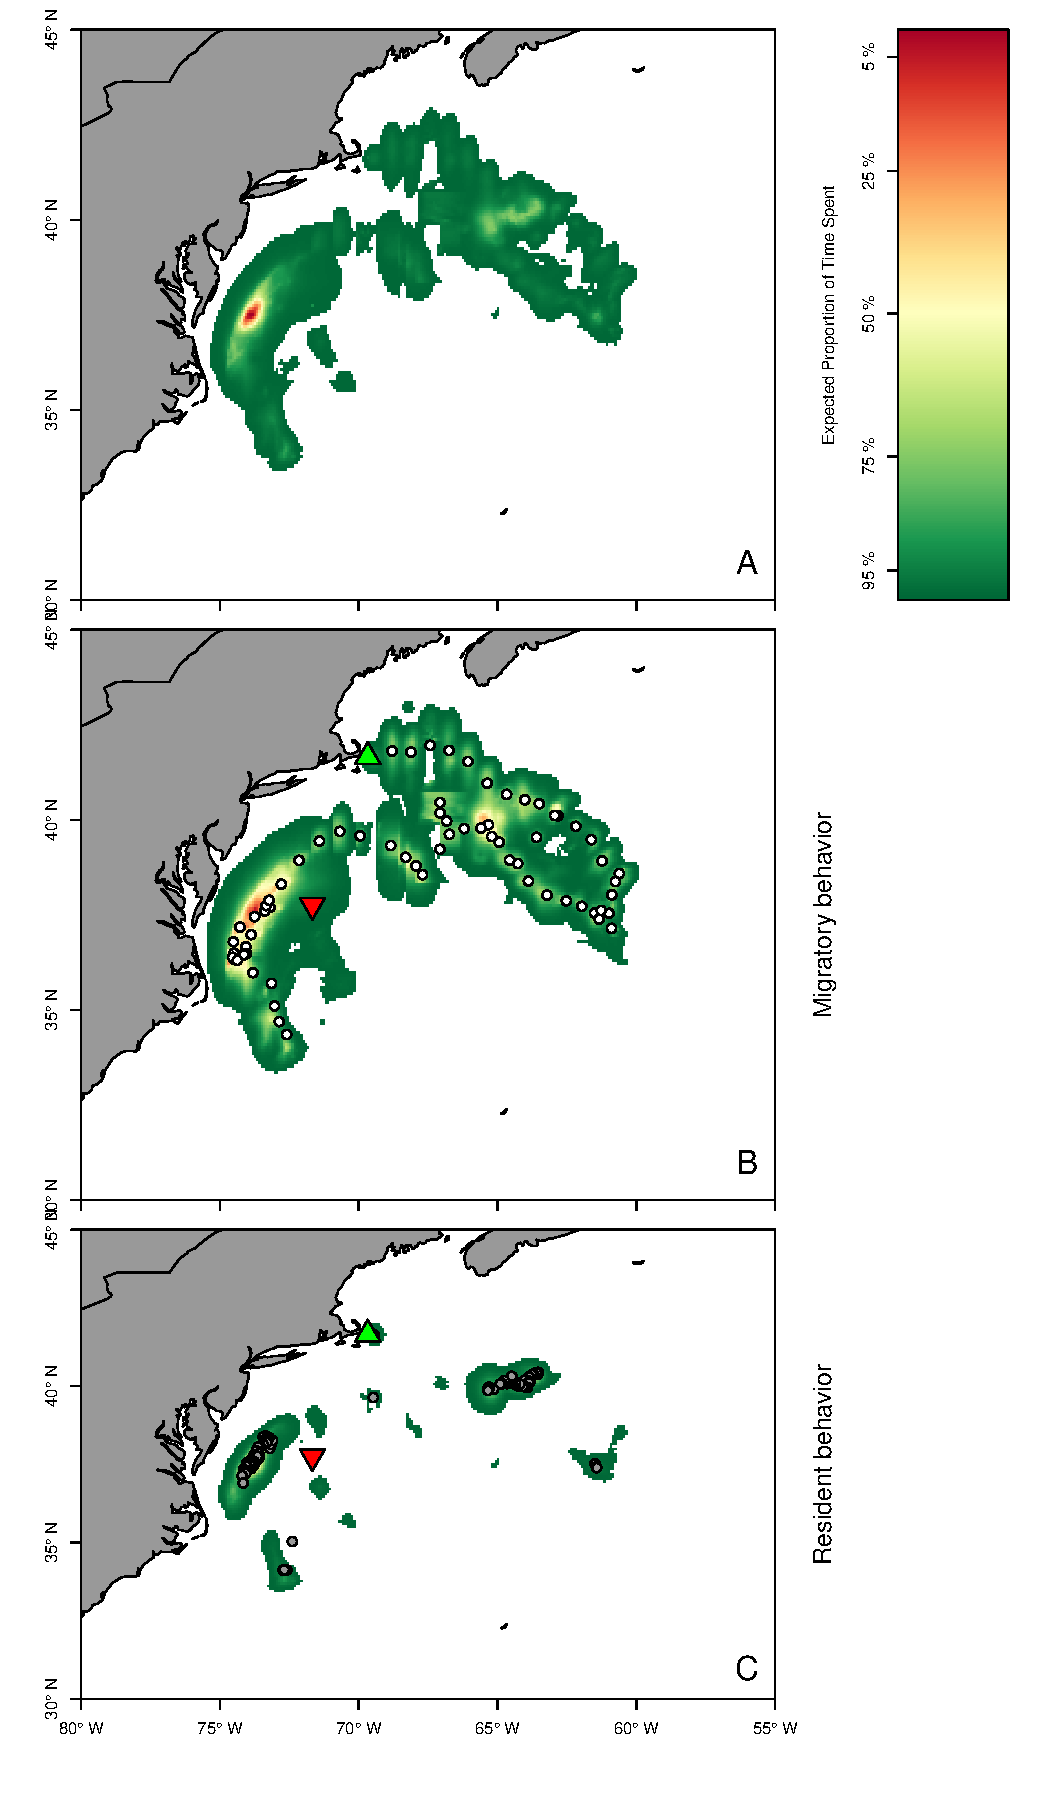
\includegraphics[width=.8\textwidth]{images/C2_Fig4.pdf}
\caption[Residency distribution results from \texttt{HMMoce}]{Residency distributions for the overall \texttt{HMMoce}
modeled movements (A) and for individual behavior states (B, C). Shaded
circles indicate residency behavior, white circles indicate migratory
behavior, green triangle is tagging location and red triangle is pop-up
location. Residency distributions show the expected proportion of time
spent in various grid cells over the course of tag deployment.}
\label{fig:c2f4}
\end{figure}


Both GPE3 and \texttt{HMMoce} provide estimated residency distributions
(RD; a form of utilization distribution) \citep{Pedersen2011}. However,
only \texttt{HMMoce} incorporates a state-switching component that
facilitates explicit modeling of distinct animal behaviors (\cref{fig:c2f3}). The state-switching is governed by movement kernels
(based on speed) and probability of switching between states is
calculated by the EM algorithm (\cref{tab:a1t1}). For the mako, the RDs
indicated areas of core use focused largely where resident behavior was
most probable. The RD for the migratory state showed the offshore
movement to the SE into the Gulf Stream region before the fish returned
to the shelf break and moved SW toward Cape Hatteras. The most notable
features of the migratory RD are the overlap areas where the fish
transitioned from migratory to resident behaviors (\cref{fig:c2f4}).

\section{Conclusions}

We present a flexible, customizable and transparent HMM framework that
may be applied to nearly any marine species utilizing electronic
archival tags through a novel use of oceanographic data. Tests of the
model demonstrated that \texttt{HMMoce} is a valuable tool for
estimating movements from low quality PSAT data through consideration of
the vertical structure of the water column in the state estimation. This
can be especially beneficial for tag data that is lacking adequate
light-level data or other measurements.

For further development, we anticipate several improvements to the
\texttt{HMMoce} package. Current priorities include support for other
tag types, direct versus derived use of light data, and additional
algorithms (\emph{e.g.} Viterbi) to calculate the most probable track
\citep{Pedersen2011}. Behavior state estimation could be expanded to
include advection or modified to update probability with respect to
environmental data \citep{Patterson2009}.

We anticipate user feedback will help prioritize further improvements,
and we welcome bug reports, feedback, and suggestions for the
development of \texttt{HMMoce} via our Github repository
\texttt{https://github.com/camrinbraun/HMMoce}. Additional usage
information, including an example dataset and a tutorial for using
\texttt{HMMoce} on Amazon Web Services, can be found by installing
\texttt{HMMoce} in \texttt{R} (\texttt{install.packages("HMMoce")}) and
accessing the package vignette.
